\documentclass[11pt]{toptesi}
%%%%%%%%%%%%%%%%%%%%%%%%%%%%%%%%%%%%%%%%%%%%%%%%%%%%%%%%%%%%%%%

% INCLUSIONE PACCHETTI
\usepackage[utf8]{inputenc} %utf8
\usepackage[italian]{babel}
%\usepackage[T1]{fontenc}
\usepackage{blindtext}
\usepackage{graphicx,wrapfig}
\usepackage{booktabs}
\usepackage{lmodern}
\usepackage{varioref}
\usepackage{url}
\usepackage{array}
\usepackage{paralist}{\obeyspaces\global\let =\space}
\usepackage{verbatim} 
\usepackage{subfig}	%per figure affiancate. Sostituisce subfigure
\usepackage{tabularx}
\usepackage{amsmath}
\usepackage{amsfonts}
\usepackage{float}
\usepackage{amssymb}
\usepackage{multicol}
\usepackage{multirow}
\usepackage{listings}
\usepackage[pass]{geometry}
\usepackage[figuresright]{rotating}
\usepackage{algorithm}
\usepackage{algorithmic}
\usepackage{amsmath}
\usepackage[babel]{csquotes}
\usepackage{hyperref}
\usepackage[backend=bibtex]{biblatex}
\usepackage{rotating}
\usepackage{tikz}
\usepackage[T1]{fontenc}
\usepackage[skip=0.01pt]{caption}


%%%%%%%%%%%%%%%%%%%%%%%%%%%%%%%%%%%%%%%%%%%%%%%%%%%%%%%%%%%%%%%

% CONFIGURAZIONE LINK E RIFERIMENTI
\hypersetup{
    pdfpagemode={UseOutlines},
    bookmarksopen,
    pdfstartview={FitH},
    colorlinks,
    linkcolor={black}, %COLORE DEI RIFERIMENTI AL TESTO
    citecolor={black}, %COLORE DEI RIFERIMENTI ALLE CITAZIONI
    urlcolor={blue} %COLORI DEGLI URL
}

%%%%%%%%%%%%%%%%%%%%%%%%%%%%%%%%%%%%%%%%%%%%%%%%%%%%%%%%%%%%%%%

% CONFIGURAZIONE LISTATI/CODICE - CANCELLARE SE NON NECESSARIO
% JAVA - BIANCO E NERO
\lstset{%
	captionpos=b,
	language=Java,
	basicstyle =\small\ttfamily,
	keywordstyle=\color{black}\bfseries,
	breaklines=true,
	breakatwhitespace=true,
	frame=lines,
	numbers=left,
	numberstyle=\footnotesize,
}

%%%%%%%%%%%%%%%%%%%%%%%%%%%%%%%%%%%%%%%%%%%%%%%%%%%%%%%%%%%%%%%

% FRENCHSPACING VA _SEMPRE_ ABILITATO PER DOCUMENTI IN ITALIANO
\frenchspacing

%%%%%%%%%%%%%%%%%%%%%%%%%%%%%%%%%%%%%%%%%%%%%%%%%%%%%%%%%%%%%%%

%DEFINIZIONE SEZIONI IN NUMERAZIONE ROMANA
%ELENCO DEI LISTATI/CODICI
\makeatletter
\newcommand\listofcodes{%
 \iffrontmatter\else\frontmattertrue\fi
 \if@openright\cleardoublepage\else\clearpage\fi
 % change the meaning of \chapter in a group
 \begingroup\def\chapter##1{\@schapter}
 \phantomsection % for the hyperlink
 \lstlistoflistings 
 \endgroup
} 
\makeatother

%%%%%%%%%%%%%%%%%%%%%%%%%%%%%%%%%%%%%%%%%%%%%%%%%%%%%%%%%%%%%%%

% INFORMAZIONI PDF - PERSONALIZZARE
\pdfinfo{%
  /Title    (Codifica video intelligente)
  /Author   (Matteo Tintori)
  /Subject  (@)
  /Keywords ( )
}
%%%%%%%%%%%%%%%%%%%%%%%%%%%%%%%%%%%%%%%%%%%%%%%%%%%%%%%%%%%%%%%


% FRONTESPIZIO - PERSONALIZZARE
% ELIMINATE LE VOCI CHE NON VI SERVONO

% UNIVERSITA - NOME
\ateneo{Università degli Studi di Firenze}

% FACOLTA - DICITURA - CANCELLARE O DECOMMENTARE
\FacoltaDi{Scuola di}
% FACOLTA - NOME
\facolta{ Ingegneria\\Dipartimento di Ingegneria dell'Informazione}

% CORSO DI LAUREA - DICITURA (MANTENERE LO SPAZIO) - CANCELLARE O DECOMMENTARE
\CorsoDiLaureaIn{Laurea Triennale in }
% CORSO DI LAUREA - NOME
\corsodilaurea{Ingegneria Informatica}

% TIPOLOGIA TESI
\TesiDiLaurea{Tesi di Laurea Triennale}

% TITOLO
\titolo{Sviluppo di sistemi per compressione video semantica\\(Development of semantic video compression system)}

% SOTTOTITOLO
%\sottotitolo{}

% RELATORE/I - DICITURA - CANCELLARE SE UN SOLO RELATORE
%\AdvisorName{Relatori}
% RELATORE - PROF. NOME E COGNOME
\relatore{Prof.Bertini Marco}

% CANDIDATO - DICITURA (MANTENERE I DUE PUNTI) - CANCELLARE O DECOMMENTARE
%\CandidateName{Candidate:}

% CANDIDATO - NOME E COGNOME
\candidato{Matteo Tintori}


% LOGO UNIVERSITA
\logosede{images/logo}

% DATA - MESE ANNO
\sedutadilaurea{Anno Accademico 2019-2020}
% LISTA DEI CAPITOLI DA INCLUDERE - PERSONALIZZARE
%\includeonly{%
%introduzione%
%}
%%%%%%%%%%%%%%%%%%%%%%%%%%%%%%%%%%%%%%%%%%%%%%%%%%%%%%%%%%%%%%%
\bibliography{bibliography}
\begin{document}
\frontespizio
%%%%%%%%%%%%%%%%%%%%%%%%%%%%%%%%%%%%%%%%%%%%%%%%%%%%%%%%%%%%%%%

%INTERLINEA - DEFAULT 1 - NON ESAGERATE, NON SUPERATE MAI 1.3 ;)
\interlinea{1.1}

%%%%%%%%%%%%%%%%%%%%%%%%%%%%%%%%%%%%%%%%%%%%%%%%%%%%%%%%%%%%%%%

\frontmatter

% DEDICA - PERSONALIZZARE
% VSPACE - PROPORZIONE USATA PER CENTRATURA VERTICALE DEL TESTO
% FLUSHRIGHT - ALLINEAMENTO ORIZZONTALE A DESTRA
\vspace*{\stretch{1}}
\begin{flushright}
\noindent
Alla mia famiglia che ha garantito economicamente in tutto il percorso di studi.\\
\vspace{1cm}
Ai compagni e agli amici che mi hanno accompagnato e in particolare a quelli che mi hanno sostenuto fino agli ultimi esami. \\
\vspace{1cm}
Al \textit{Prof. Bertini Marco} per la professionalità e risolutezza nel fornire ogni tipo di materiale e aiuto.
\end{flushright}
\vspace*{\stretch{6}}
\cleardoublepage


% CITAZIONE - PERSONALIZZARE
% VSPACE - PROPORZIONE USATA PER CENTRATURA VERTICALE DEL TESTO
% FLUSHRIGHT - ALLINEAMENTO ORIZZONTALE A DESTRA
\vspace*{\stretch{1}}
\begin{flushright}
\noindent
La pazienza è amara, ma dolce è il suo frutto. \\
\textit{(Jean-Jacques Rousseau)}
\end{flushright}
\vspace*{\stretch{6}}
\cleardoublepage

%%%%%%%%%%%%%%%%%%%%%%%%%%%%%%%%%%%%%%%%%%%%%%%%%%%%%%%%%%%%%%%
% RINGRAZIAMENTI - PERSONALIZZARE
%\ringraziamenti


%%%%%%%%%%%%%%%%%%%%%%%%%%%%%%%%%%%%%%%%%%%%%%%%%%%%%%%%%%%%%%%

% INDICI - ELIMINARE GLI INDICI NON NECESSARI

% INDICE GENERALE
\tableofcontents

% INDICE DELLE FIGURE
\listoffigures

%% INDICE DELLE TABELLE
%%\listoftables

%% INDICE DEI CODICI
%%\listofcodes

%%%%%%%%%%%%%%%%%%%%%%%%%%%%%%%%%%%%%%%%%%%%%%%%%%%%%%%%%%%%%%%

\mainmatter

% INCLUSIONE FILE CAPITOLI - PERSONALIZZARE - TENERE COERENTE CON LISTA IN ALTO
\chapter{Introduzione}
\label{chap:intro}
%Introduzione su cosa ho fatto

\section{Intento}
\label{sec:intento}
%Identifica il prodotto, includendo versione di revisione e/o rilascio. 

L'obbiettivo di questo elaborato è la realizzazione di un Codec a partire da formato \textbf{H.265} destinato a video di calcio HD, che performi una compressione altrettanto efficiente ma variabile sulla base del contenuto interessante di ogni singolo frame.
In particolare, si vuole codificare una partita di calcio utilizzando reti neurali convoluzionali per il riconoscimento e la conseguente segmentazione dei giocatori sul campo, e quando possibile, della palla. 
Le posizioni delle suddette entità sono le regioni di interesse che saranno lasciate senza perdita di qualità, mentre sulle altre zone verrà applicato un filtro che fornirà una compressione migliore "sacrificando" le alte frequenze e quindi una piccola parte di informazione non interessante. Viene poi effettuato un confronto tra il video originale e quello codificato come indice di efficienza, utilizzando metriche di qualità oggettiva. Infine, come indice di miglior codifica, viene effettuato un confronto tra i risultati di questo prodotto e un altro prodotto basato su Codec x264 e salienza, intesa come punto centrale dove l'osservatore è abituato a guardare spontaneamente, e se ne deduce il migliore in termini di dimensioni del prodotto compresso risultante.


\section{Ambito del progetto}
\label{sec:projscope}
%Breve descrizioni del software , includendo benefici, obiettivi e goals.
Il software si colloca nel campo della computer vision e si vuole affermare come Codec \textbf{H.265} che punta a comprimere più informazioni delle librerie già usate, valido particolarmente nei casi in cui ci sia una limitazione di spazio nel device in cui si scarica/guarda il video o nel caso si debba risparmiare per motivi economici sulla quantità di dati scaricati (ad esempio una soglia di (G)byte massima fissata dal gestore telefonico). 
Il Codec non si propone come versione superiore delle implementazioni già esistenti di \textbf{H.265} ma piuttosto come alternativa semantica.
\\
\chapter{Strumentazione}
\label{chap:tools}

\section{Piattaforma di sviluppo}
\label{sec:platform}
La workstation usata per lo sviluppo del software è un server Linux con 2 schede video NVIDIA Titan X ed è collegata alla rete con IP pubblico all'indirizzo solaris.micc.unifi.it ed accedibile con utente mtintori. 
La modalità di lavoro perseguita è remota utilizzando remote desktop da PC Windows e PC Mac in seguito.
L'IDE utilizzato per lo sviluppo è Pycharm con versione di Python 3.6.

\section{Miniconda}
Miniconda è un gestore di pacchetti ed environment-manager. E' una versione di installazione minimale di Anaconda, comprende l'interprete Python e permette di utilizzare un'IDE alternativo a Spider, usato con Anaconda, inoltre non vengono installati gli oltre 250 pacchetti che sono compresi nell'installazione di Anaconda lasciando la libertà allo sviluppatore su quali pacchetti installare.
\label{sec:miniconda}
\subsection*{Ambienti Miniconda}
Utilizzeremo il termine Conda, istruzione fondamentale Miniconda, per riferirsi al sunnominato manager.
Per la realizzazione del Codec si è resa necessaria la creazione di due ambienti Conda: è stata effettuata una simile scelta per possibilità di debug anche in assenza di rete su una workstation personale che non possiede una GPU. 
\begin{itemize}
\item \emph{tf\_cpu} : ambiente più lento, ma utilizzabile anche da una workstation non avente GPU
\item \emph{tf\_gpu} : ambiente più veloce, ma utilizzabile solo da una workstation con una GPU con ampia memoria adatta al training di reti neurali
\end{itemize}
\section{Schema del sistema}
\begin{figure}
   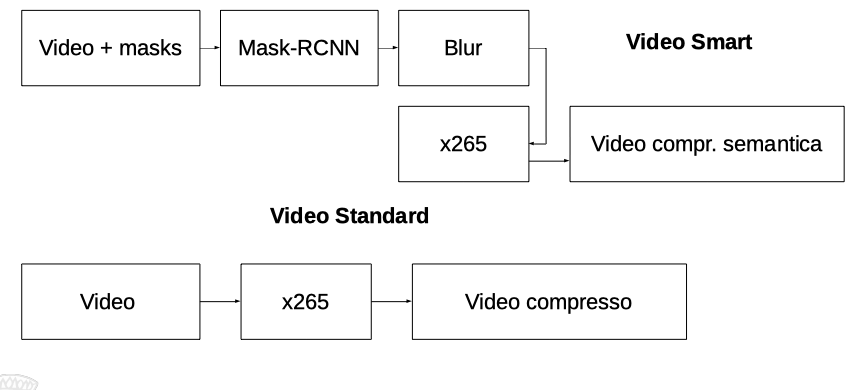
\includegraphics[width=\linewidth]{images/schema.png}
   \caption{}
   \label{fig:c}
\end{figure}
\section{CODEC di partenza}
\label{sec:codec_base}
%Descrivere il codec
La scelta del codec da utilizzare era contesa tra gli standard candidabili \textbf{H.264}, \textbf{H.265}, mentre gli altri due standard ottimali \textbf{VP9} e \textbf{AV1} non sono stati volontariamente presi in considerazione come assunto iniziale, nonostante le performance del secondo qualche volta superiore a \textbf{H.265} implementato dall'encoder \textbf{x265}.\textsuperscript{\ref{fig:c}} (si noti che \textbf{VP9} invece è visibilmente inferiore agli altri,come si nota pur dalle info \textbf{libvpx}\textsuperscript{\cite{libvpx}} che lo implementa).
\begin{figure}
   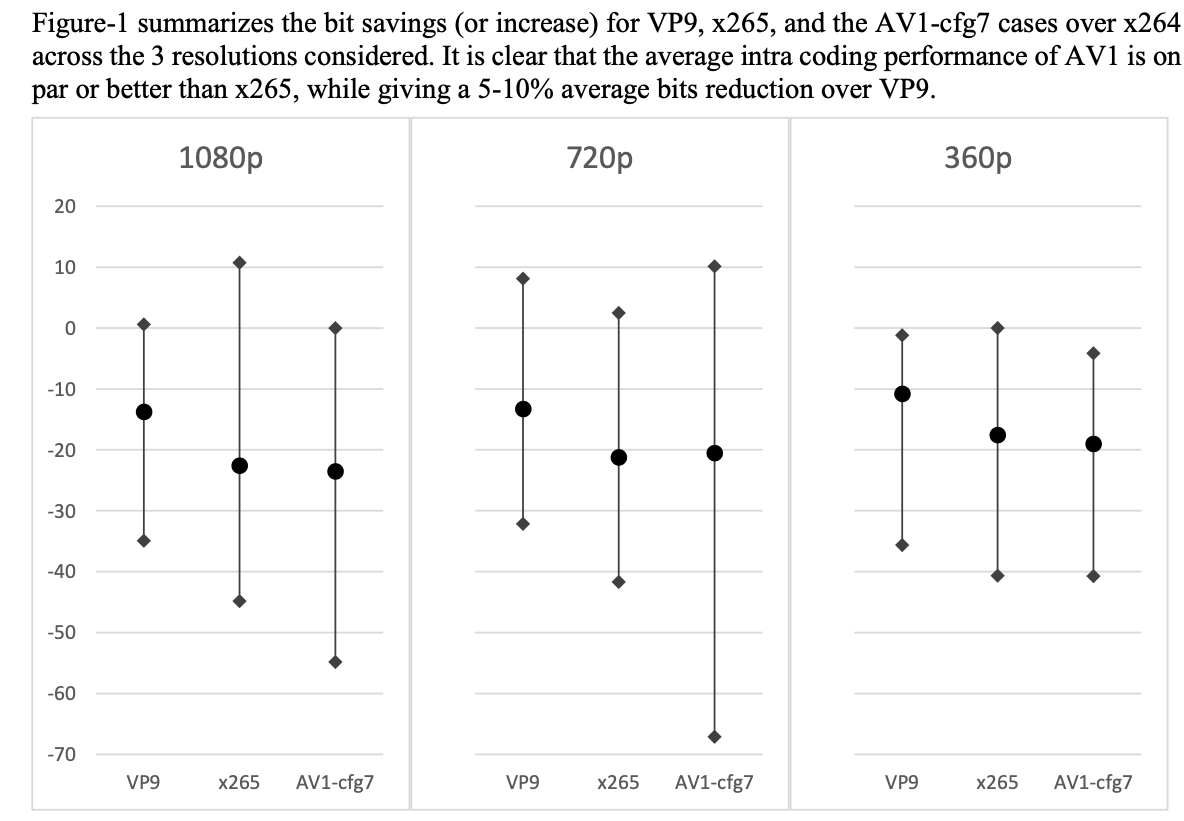
\includegraphics[width=\linewidth]{images/x265vsAv1.png}
   \caption{Risparmio in bits (segni: - risparmio, + incremento)}
   \label{fig:c}
\end{figure}
\\Sappiamo anche che \textbf{x264} implementa lo standard precedente; è quindi sicuramente più scarso. Lo standard dalla quale siamo partiti per una codifica efficiente è allora \textbf{H.265} usando \textbf{hevc\_nvenc} \textsuperscript{\ref{sec:nvenc}}, ed abbiamo optato per una codifica progressiva frame per frame. Il nostro encoder prevede una quantizzazione "doppia", poiché prima di scrivere ogni frame vengono selezionate le regioni non interessanti e ne vengono tagliate fuori le HF\footnote{Alte frequenze}; ciò verrà spiegato in seguito. Quello che invece fa il Codec di partenza che abbiamo scelto è una quantizzazione secondo lo standard, che viene effettuata manovrando il parametro \emph{QP} cui valore rappresenta la sua intensità, ovvero quanta informazione (sempre HF) viene scartata.
\subsection*{CRF}
Il Costant Rate Factor\textsuperscript{\cite{CRF_vs_QP}}  è un fattore che influenza la quantizzazione in modo più sofisticato del parametro a basso livello \emph{QP} previsto dallo standard H.265. Più alto il CRF, più i campioni (pixel o blocchi di pixel) vengono quantizzati in maniera maggiore; questo valore resta fisso per l'intera codifica del video scelto, mentre il valore del parametro \emph{QP} varia a seconda di quanto si debba quantizzare in ogni frame per mantenere una qualità costante.
Nel nostro caso, utilizzando \textbf{nvenc} non sarà presente il parametro \emph{crf} ma si deve utilizzare il parametro equivalente \emph{cq} di questa libreria a cui sarà dato un valore che garantirà una compressione visivamente lossless, ovvero con perdita di qualità trascurabile all'occhio umano; essenzialmente questo valore per \textbf{h264\_nvenc} è circa 19 per cui, preso atto che il valore di default di \textbf{x264} è 23 e corrisponde a circa 28 di \textbf{x265}, non sbaglieremo nel dire che 19 è sicuramente visually lossless anche per \textbf{hevc\_nvenc}.
\section{FFMPEG}
\label{sec:coding_library}
%Descrivere il codec
Utilizzando la libreria \textbf{FFMPEG} è stato possibile scegliere diversi parametri oltre al Codec \textbf{hecv\_nvenc}. 
Le modalità tipiche di codifica sono 3: \footnote{vedi rate control modes: https://trac.ffmpeg.org/wiki/Encode/H.265} 
\begin{enumerate}
\item bitrate scelto in 1 passo (sconsigliato)
\item bitrate scelto in 2 passi
\item CRF (fattore di qualità costante)
\end{enumerate}
Dal momento che non è nostro interesse il raggiungimento di una dimensione file particolare, la scelta è caduta sulla terza opzione, che è stata spiegata nella sottosezione precedente.
Gli altri parametri che abbiamo utilizzato per la codifica sono i seguenti:
\begin{itemize}
\item \textbf{-cq}: fattore di qualità che mantiene la suddetta costante in ogni frame manovrando il parametro che definisce la quantizzazione \emph{QP}
\item \textbf{-qmin} : fattore minimo di qualità che \textbf{cq} può assumere
\item \textbf{-qmax} : fattore massimo di qualità che \textbf{cq} può assumere
\item \textbf{-b:v} : posto a 0 per causa di un bug nella libreria, che se non venisse settato inibisce il funzionamento di cq
\item \textbf{-rc} : rate control, sovrascrive la velocità di compressione ("preset",più basso il preset più alta la qualità) e deve essere settato insieme a \textbf{\emph{-b:v}} per una qualità costante
\item \textbf{-r} : frame rate, ovvero quanti frame vengono campionati nell'unità di tempo
\end{itemize}
%Descrivere l'ambiente in cui opererà il software, includendo piattaforme hardware, altri sistemi operativi con relativa versione, altre componenti software che utilizza questo prodotto

\section{Mask-RCNN}
\label{sec:Mask-RCNN_desc}
Mask-RCNN è un'implementazione di una rete neurale Faster-RCNN da parte del framework tensorflow di Google. Si differenzia dalle Faster-RCNN per l'introduzione del RoI Align, più preciso rispetto al RoI Pooling precedente. Facciamo un piccolo riepilogo per maggiore chiarezza.
\subsection*{Riepilogo - Dalle CNN alle Faster-RCNN}
Le reti neurali convoluzionali \textbf{(CNN)} sono state introdotte nel campo dell' IA per vari scopi e più precisamente nella computer vision sono utili per il riconoscimento di qualsiasi entità o pattern all'interno di un immagine. Le potenzialità e i limiti sono elencati di seguito:
\begin{enumerate}
\item Usano una funzione softmax per classificazione multi-classe e sigmoid per classificazione binaria
\item Usata per image classification e object detection
\item Rileva solo un oggetto alla volta senza sovrapposizioni
\end{enumerate}
Successivamente si sono affermate le CNN basate su regioni \textbf{(RCNN)}, che forniscono il miglioramento di riconoscere più oggetti diversi nella stessa immagine e identificarli all'interno di un rettangolo. Questo è possibile con il seguente procedimento:
\begin{enumerate}
\item Generazione di regioni propositive con R-CNN per mezzo dell'algoritmo \emph{Selective Search} unito con \emph{Exhaustive Search}
\item Fusione di regioni propositive simili e \emph{Feature extraction} con CNN per ogni regione propositiva
\item Algoritmo \emph{Support vector machine} per la feature estratta per la verifica dell'effettiva presenza dell'oggetto 
\item Algoritmo \emph{Non-Max suppression} per lo scarto di regioni con basso punteggio in \emph{Intersection over Union}.
\end{enumerate}
Per ottenere un altro significativo miglioramento siamo arrivati alle reti \textbf{Fast-RCNN}, che offrono i seguenti vantaggi:
\begin{enumerate}
\item Unica rete neurale (deep ConvNet) che sostituisce quelle migliaia di R-CNN sulle singole regioni
\item Unico modello per la feature extraction, la classificazione e le bounding boxes
\item Introduzione delle Region of Interest (RoI) e del RoI Pooling
\end{enumerate}
Infine, si è voluto perfezionare l'arte del riconoscimento e identificazione delle forme di ogni entità con le reti \textbf{Faster-RCNN}, che permettono di:
\begin{enumerate}
\item 3-D object detection
\item Part-based detection
\item Instance segmentation
\item Image captioning
\end{enumerate}




\chapter{Analisi}
\label{chap:analysis}
Il codec descritto, non è utiizzabile come versione stand-alone integrata in un software applicativo, ma potrà essere dispiegata come estensione chrome o browser alternativo in modo che sia fruibile sia da PC che da Smartphone e utilizzabile ogni qual volta viene scaricato un video con qualità almeno 720p. 
\section{Analisi Funzionale}
\label{sec:func}
Su questo tipo di analisi è necessario essere brevi, perché l'unica funzionalità offerta dall'encoder è appunto su richiesta dell'utente scaricare o visionare il video 720p o 1080p nel nostro formato H.265.
Le funzionalità descritte possono essere fruite nei seguenti modi:
\begin{itemize}
\item Installando come estensione browser il nostro progetto encoder e selezionando l'opzione "SI" al popup in apertura dopo il click del download.
\item Il nostro Codec verrà fornito nella lista delle risoluzioni di un video visionabile elencandolo come 720p e 1080p "ottimizzato", e verrà caricato alla scelta con la codifica in questione. 
\end{itemize}
Di seguito abbiamo previsto un'immagine utilizzata esclusivamente per documentare la metodologia del lavoro svolto di riconoscimento e segmentazione dei giocatori su un particolare frame:
\begin{figure}
   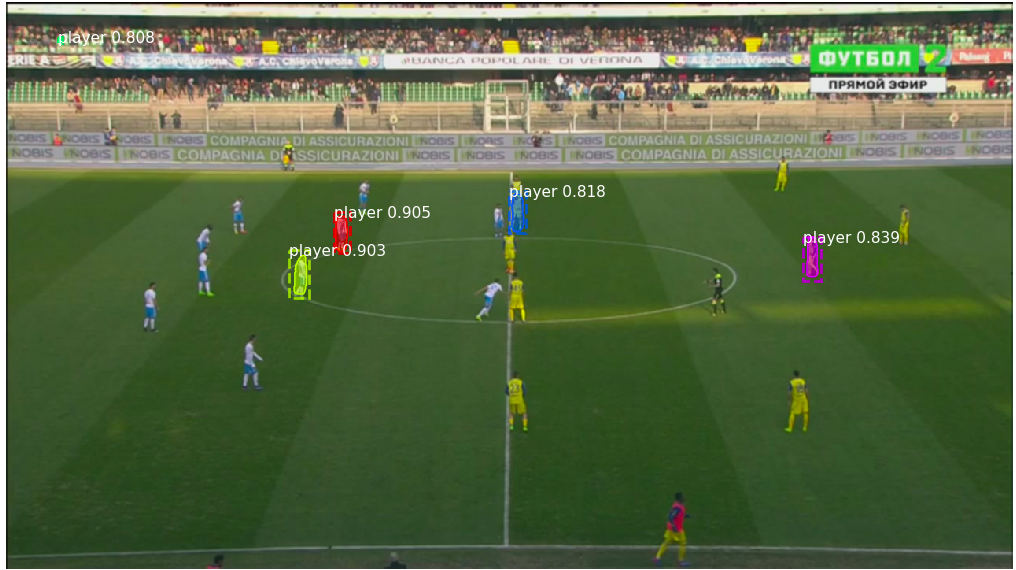
\includegraphics[width=\linewidth]{images/dim.png}
   \caption{dimostrazione di segmentazione giocatori}
   \label{fig:dim}
\end{figure}
\newpage
\section{Analisi Tecnica}
\label{sec:tech}
I file scritti personalmente che fanno parte di questo progetto sono 4 e ha anche una particolare importanza il file model.py non implementato personalmente, in quanto contiene la struttura di tutta la rete neurale da cui possiamo trarre i metodi per la creazione dell'oggetto che rappresenta la rete e per effettuare il training di essa.
\begin{itemize}
\item fine\_tuning.py
La classe è stata introdotta con la responsabilità di effettuare tutte le operazioni di training e di fine tuning della nostra rete e instanziare un oggetto soccer\_dataset su cui far partire due training: il primo sui top layers chiamati \emph{heads} e il secondo sui livelli \emph{4+} ovvero dallo strato 4 in su di una rete ResNet101. Questo è stato fatto attenendosi ad alcune fonti \textsuperscript{\cite{fine_tuning_book}}  e all'esempio \emph{balloon.py} poiché potevamo scegliere di fare un fine tuning sbloccando per l'allenamento anche solo i livelli più vicini agli heads: \emph{5+} oppure più lontani dagli heads: \emph{3+} o perfino allenare la rete totalmente.
\item soccer\_dataset.py
Carica un dataset di immagini di annotazioni in formato pascalVOC
\item main.py
Si occupa di gestire l'input della barra di comando che deve essere un video HD che mostra una partita di calcio, ne effettua l'instance segmentation, la quantizzazione e codifica per produrre un video Mp4 codificato H.265 con LPF.
\item clever\_config.py
Specifica la configurazione delle impostazioni di fine tuning desiderate che devono essere passate alla classe omonima per almeno i parametri fondamentali quali STEP\_PER\_EPOCH,GPU\_COUNT,NUM\_CLASSES oppure BATCH\_SIZE nel caso di parametro IMAGES\_PER\_GPU maggiore di 1.
\end{itemize}
Alla pagina seguente si riassume la struttura del progetto utilizzando un diagramma UML.

\subsection*{Main}
Come si può osservare dalla struttura del file main.py, questo non contiene una classe bensì un'istruzione che si accerta che il file main sia eseguito da riga di comando come primo file, e non sia quindi importato da altri files.
L'espressione che rende un booleano per confermare questa condizione è la seguente: \textbf{\_\_name\_\_ == "\_\_main\_\_"}
Come visibile dal diagramma UML collocato in seguito, il file main offre i seguenti metodi:
\begin{itemize}
\item Un metodo \emph{draw\_images\_with\_boxes} che si propone come metodo di "debug" in quanto serve solamente a mostrare il lavoro di riconoscimento e segmentazione svolto quando l'input è un'immagine, cosa che esula dai nostri obbiettivi di codifica \textbf{video}.
\item Un metodo \emph{is\_video\_file} che prende in ingresso un estensione e la confronta con tutte le esistenti estensioni video per capire se l'input in ingresso è effettivamente un video o meno.
\item Un metodo \emph{quantize\_frame} che è il metodo fulcro della nostra codifica per Region of Interest (RoI), infatti utilizza una copia del frame e vi applica un filtro passa-basso per rimuoverne le HF, dopodiché incolla le maschere dei giocatori del frame originale che le contiene ancora in HD sul frame copia, facendo risultare l'effetto LPF solo sulle regioni di non interesse.
\item Il metodo  \emph{main} che è il metodo contenente tutto il codice utile per arrivare ai seguenti risultati:
\begin{enumerate}
\item Ottenere i parametri inseriti a barra di comando
\item Controllare se c'è un parametro(booleano) fine tuning attivo e in caso affermativo delegare la responsabilità di effettuare il training alla classe omonima
\item Controllare se c'è un parametro input e in caso affermativo controllare se l'input è un video: in caso negativo se è un immagine la visualizza a video come instance segmentation
\item In caso che invece il parametro di input sia un video instanzia un oggetto \textbf{FFMpegWriter} con l'encoder \textbf{hevc} e con un coefficente di qualità costante adatto, dopodiché ne cicla i frame uno per uno
\item Una volta dentro il ciclo utiizza la funzione \emph{quantize\_frame} per applicare un LPF al frame corrente, dopodiché lo scrive nel nuovo video con la funzione \emph{write} di \textbf{FFMpegWriter}
\item Alla fine del ciclo, tutti i frame sono stati scritti in modo codificato "2 volte", ovvero una grazie all'oggetto \textbf{FFMpegWriter} che ha tolto una quantità di informazioni trascurabile e l'altra grazie al nostro LPF. Infine quindi le risorse vengono rilasciate e il nuovo video viene salvato con estensione contenitore generica .mp4
\end{enumerate}
\end{itemize}
\subsection*{Classe model}
La descrizione di ciò che le classi operano è riassunta nel preambolo di questa sezione, essendo esse strettamente collegate ai rispettivi files in python. Descriviamo ora in particolare la classe non implementata da noi denominata \emph{model} che chiameremo con il suo alias \emph{modellib} e il suo utilizzo, dopodiché ci soffermiamo su attributi e metodi delle classi corrispondenti ai files già descritti in precedenza.
Come visibile dal diagramma UML collocato in seguito, la classe modellib all'interno di model.py deve offrire:
\begin{itemize}
\item Un attributo accessibile dal model che rappresenta i pesi\emph{(weights)} allenati della rete, accessibile come keras\_model.history.history
\item Un costruttore statico utilizzabile con l'istruzione modellib.MaskRCNN che restituisce un'istanza del model.
\item Un metodo che viene usato per caricare i \emph{weights} escludendo i 4 layers che comprendono la lista di tutte le labels su cui è stata allenata originariamente la rete MaskRCNN, in modo da personalizzare il training su esclusivamente i giocatori e la palla, denominato \emph{load\_weights.}
\item Un metodo denominato \emph{train} che consente effettivamente di effettuare il training dei \emph{weights} specificando il training set e il test set, i layers bersaglio che devono essere sbloccati per il fine tuning(heads o 3/4/5+),il numero di epochs e il learning rate che vengono ricavati dal file clever\_config.py per best practice e le trasformazioni casuali sui frames (\emph{augmentation}) per un allenamento dinamico.
\item Un metodo denominato \emph{save\_weigths} che viene utilizzato per salvare sul file system i \emph{weights} addestrati dopo il fine tuning e viene richiamato con keras\_model.save\_weigths.
\end{itemize}

\subsection*{Classe SoccerDataset}
La classe SoccerDataset ridefinisce i metodi della sua superclasse Dataset,eccetto un metodo che merita una menzione particolare chiamato \emph{prepare}, che presa per scontata l'equivalenza tra labels e classi,offre le seguenti operazioni:
\begin{itemize}
\item Il metodo suddetto  salva tutte le informazioni delle classi come il numero e il nome di esse, compresi gli IDs in forma autoincrementante dalla variabile \emph{self.class\_info}
\item Mappa IDs interni(class e images) partendo dalle info come \emph{self.class\_info} e \emph{self.class\_ids}
\item Mappa i sorgenti(sources) verso i class\_ids che essi supportano.
\end{itemize}
Il metodo che è sottoposto a ovveride nella classe figlia chiamato \emph{load\_dataset}, come si può osservare dal nome autodocumentante, si limita a caricare le classi del dataset personalizzato.
Gli altri metodi, che non sono sottoposti a override ma sono totalmente nuovi nella classe figlia SoccerDataset, sono elencati seguentemente con i loro effetti:
\begin{itemize}
\item extract\_polygons : è il metodo fondamentale per la lettura delle annotazioni JSON di un immagine scelta che contengono le informazioni sui poligoni che descrivono i giocatori e la decodifica dei dati su di essi per poi essere salvati in un array di polygons che sarà restituito al chiamante insieme alla larghezza e all'altezza dell'immagine.
\item load\_mask : il metodo corrente, data un'ID intera di un'immagine, restituisce la sua altezza,larghezza e l'array di poligoni che sono stati estratti con il metodo \emph{extract\_polygons}
\item image\_reference : ritorna la path del'immagine 
\end{itemize}

\subsection*{Classe FineTuning}
La classe sunnomminata si dedica innanzitutto a creare una configurazione personalizzata CleverConfig che sarà utilizzata nella stessa classe come parametro per costruttore del model, nell'unico metodo esistente che è:
\begin{itemize}
\item start: questo metodo si dedica alla creazione dei train\_set e test\_set per l'allenamento della rete, alla creazione dell'oggetto model per il caricamento dei pesi e per il loro allenamento in 2 fasi: prima quello degli \emph{heads} e successivamente quello dei livelli \emph{4+}
\end{itemize}
\subsection*{Classe CleverConfig}
Effettua l'ovverride della classe Config standard che è anonima ma contiene tutti i parametri per effettuare un fine tuning o training da una rete blackbox, ovvero che non ha ricevuto nessun addestramento.\\
I parametri con cui la classe Config se non ridefinita performerebbe il training della rete sono i seguenti(trascritti direttamente dalla classe config.py):\\

\begin{lstlisting}
class Config(object):

 
    NAME = None  # Override in sub-classes

    GPU_COUNT = 1

  
    IMAGES_PER_GPU = 2

    STEPS_PER_EPOCH = 1000

  
    VALIDATION_STEPS = 50

    BACKBONE = "resnet101"

    COMPUTE_BACKBONE_SHAPE = None

    # The strides of each layer of the FPN Pyramid. These values
    # are based on a Resnet101 backbone.
    BACKBONE_STRIDES = [4, 8, 16, 32, 64]

    # Size of the fully-connected layers in the classification graph
    FPN_CLASSIF_FC_LAYERS_SIZE = 1024

    # Size of the top-down layers used to build the feature pyramid
    TOP_DOWN_PYRAMID_SIZE = 256

    # Number of classification classes (including background)
    NUM_CLASSES = 1  # Override in sub-classes

    # Length of square anchor side in pixels
    RPN_ANCHOR_SCALES = (32, 64, 128, 256, 512)

    # Ratios of anchors at each cell (width/height)
    # A value of 1 represents a square anchor, and 0.5 is a wide anchor
    RPN_ANCHOR_RATIOS = [0.5, 1, 2]

    # If 1 then anchors are created for each cell in the backbone feature map.
    # If 2, then anchors are created for every other cell, and so on.
    RPN_ANCHOR_STRIDE = 1

    # Non-max suppression threshold to filter RPN proposals.
    # You can increase this during training to generate more propsals.
    RPN_NMS_THRESHOLD = 0.7

    # How many anchors per image to use for RPN training
    RPN_TRAIN_ANCHORS_PER_IMAGE = 256
    
    # ROIs kept after tf.nn.top_k and before non-maximum suppression
    PRE_NMS_LIMIT = 6000

    # ROIs kept after non-maximum suppression (training and inference)
    POST_NMS_ROIS_TRAINING = 2000
    POST_NMS_ROIS_INFERENCE = 1000

    # If enabled, resizes instance masks to a smaller size to reduce
    # memory load. Recommended when using high-resolution images.
    USE_MINI_MASK = True
    MINI_MASK_SHAPE = (56, 56)  # (height, width) of the mini-mask

    IMAGE_RESIZE_MODE = "square"
    IMAGE_MIN_DIM = 800
    IMAGE_MAX_DIM = 1024
  
    IMAGE_MIN_SCALE = 0
       IMAGE_CHANNEL_COUNT = 3

    # Image mean (RGB)
    MEAN_PIXEL = np.array([123.7, 116.8, 103.9])

       TRAIN_ROIS_PER_IMAGE = 200

    # Percent of positive ROIs used to train classifier/mask heads
    ROI_POSITIVE_RATIO = 0.33

    # Pooled ROIs
    POOL_SIZE = 7
    MASK_POOL_SIZE = 14

    # Shape of output mask
    # To change this you also need to change the neural network mask branch
    MASK_SHAPE = [28, 28]

    # Maximum number of ground truth instances to use in one image
    MAX_GT_INSTANCES = 100

    # Bounding box refinement standard deviation for RPN and final detections.
    RPN_BBOX_STD_DEV = np.array([0.1, 0.1, 0.2, 0.2])
    BBOX_STD_DEV = np.array([0.1, 0.1, 0.2, 0.2])

    # Max number of final detections
    DETECTION_MAX_INSTANCES = 100

    DETECTION_MIN_CONFIDENCE = 0.7

    # Non-maximum suppression threshold for detection
    DETECTION_NMS_THRESHOLD = 0.3

  
    LEARNING_RATE = 0.001
    LEARNING_MOMENTUM = 0.9

    # Weight decay regularization
    WEIGHT_DECAY = 0.0001

    LOSS_WEIGHTS = {
        "rpn_class_loss": 1.,
        "rpn_bbox_loss": 1.,
        "mrcnn_class_loss": 1.,
        "mrcnn_bbox_loss": 1.,
        "mrcnn_mask_loss": 1.
    }
    
    USE_RPN_ROIS = True

    TRAIN_BN = False  # Defaulting to False since batch size is often small

    # Gradient norm clipping
    GRADIENT_CLIP_NORM = 5.0
\end{lstlisting}

Per effettuare quindi un fine tuning addatto all'evenienza abbiamo ridefinito i seguenti parametri, con il nostro ovveride della classe Config:
\begin{lstlisting}
class CleverConfig(Config):
    # give the configuration a recognizable name
    NAME = "clever_coding_config"

    # set the number of GPUs to use along with the number of images
    # per GPU
    GPU_COUNT = 1
    IMAGES_PER_GPU = 1
    # Skip detections with < 90% confidence
    DETECTION_MIN_CONFIDENCE = 0.8
    # batch_size=2. Samples=50. steps=50/2
    STEPS_PER_EPOCH = 120
    VALIDATION_STEPS = 25
    BATCH_SIZE = 1 #GPU_COUNT*IMAGES_PER_GPU
    # number of classes (we would normally add +1 for the background
    # but the background class is *already* included in the class
    # names)
    NUM_CLASSES = 1 + 2

\end{lstlisting}
\newpage
\begin{sidewaysfigure}
   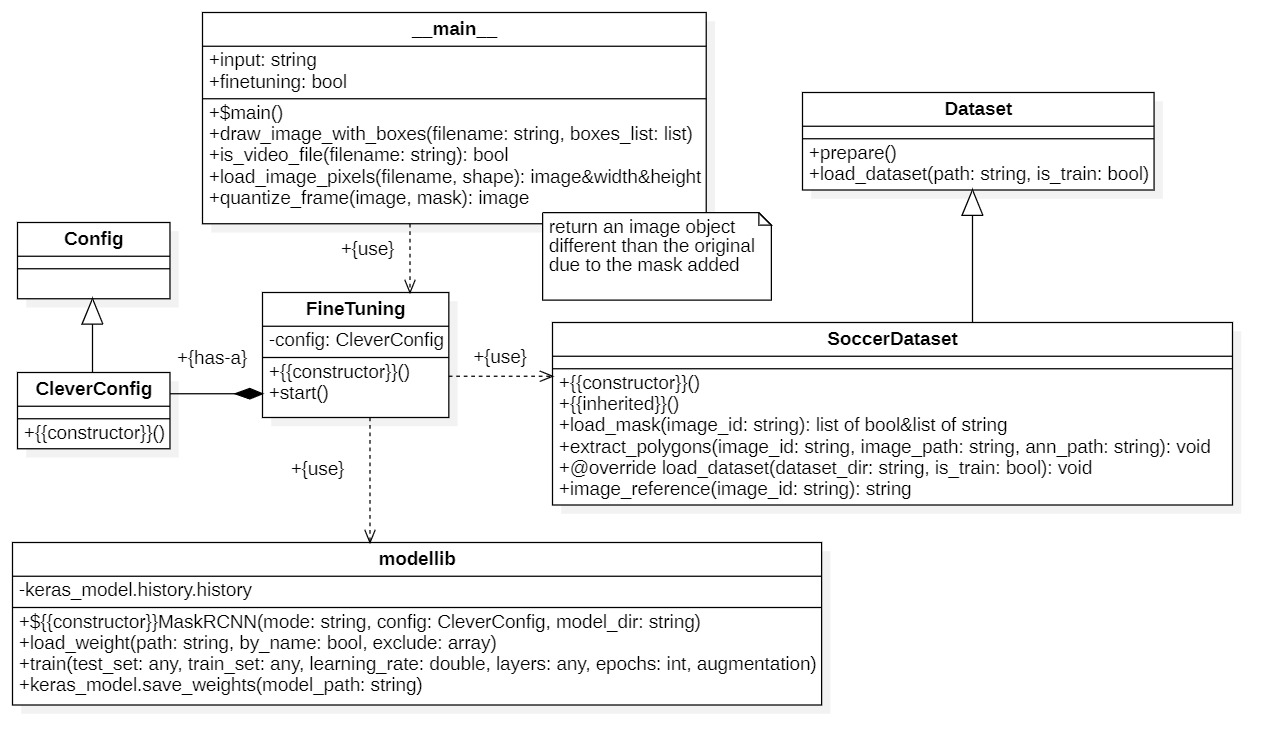
\includegraphics[width=\linewidth]{images/UML.jpg}
    \caption{Diagramma UML del progetto}
    \label{fig:uml}
\end{sidewaysfigure}







\chapter{Sistema di segmentazione oggetti}
\label{chap:preparation}
In questo capitolo, per iniziare, si vuole distinguere la differenza tra un training di una rete blackbox e un fine tuning di una rete preaddestrata.\\
Essendo \textbf{Mask-RCNN} una rete preaddestrata per circa 60 classi, si parlerà innanzitutto di un fine tuning e non di un allenamento di una rete partendo da zero esperienza(blackbox).\\
La cosa che distingue il nostro agire in questo caso è che faremo un fine tuning, non sulle circa 60 classi sulla quale è stata preaddestrata la rete, ma solamente su 2 classi che rappresenteranno i giocatori e la palla all'interno del campo di calcio.
\newpage
\section{Strutturazione Fine-Tuning}
Come premessa, bisogna dichiarare il fatto che per un buon fine tuning serve scegliere un software di labeling che fornisce le annotazioni in un certo formato, solitamente XML.
Nel nostro caso, siccome sappiamo che PASCALVOC XML viene usato quando c'è da fare object detection mentre noi cerchiamo di fare instance segmentation, abbiamo usato un software chiamato \textbf{labelme} che produce annotazioni con estensione JSON in modo da prelevare facilmente i dati dei poligoni racchiusi nei files.
Lo strumento \textbf{labelme} viene utilizzato per tracciare poligoni intorno ai giocatori nei frames, cioè le immagini singole di un video che è stato frammentato con uno strumento come ad esempio \textbf{Avidemux}. \\
Nel software \textbf{labelme} quando viene scelto un tracciamento della curva \emph{poligono}, questi poligoni devono essere tracciati come linea spezzata chiusa con un numero di punti adatto a circondare con la minima tolleranza possibile la forma di un giocatore, e nel caso della scelta sul software \textbf{labelme} della curva \emph{cerchio}, esso andrà a circondare la palla.
Chiaramente, un giocatore potrà essere all'interno del campo in diverse posizioni, ad esempio in piedi fermo, in piedi in corsa oppure a terra come dopo una parata o una scivolata; tutti questi casi devono essere circondati da punti che formano un poligono per far sì che la rete \textbf{MaskRCNN} abbia un allenamento soddisfacente.\\
Una volta salvato il frame modificato con i poligoni, il software \textbf{labelme} genererà un file JSON con all'interno i dati del nome dell'immagine, la sua altezza e larghezza, il numero e i punti dei poligoni in modo da essere letti successivamente da codice.
L'operazione di contornamento dei giocatori e della palla con i poligoni di punti, si chiama \textbf{labeling}, e si può effettuare un labeling anche massivo specificando all'apertura del software \textbf{labelme}  una directory dove sono presenti tutti i frames del video obbiettivo e in contempo una directory vuota dove produrre in massa i file JSON delle loro annotazioni; ogni file di annotazione viene prodotto non appena il labeling di un immagine viene ultimato e quindi l'immagine viene salvata.
\chapter{Discussione}
\label{chap:discussion}

\section{Commenti al Codice}
\label{sec:comments}
\begin{enumerate}
\item Partendo dal principio, analizziamo la riga \emph{get\_ipython} e \emph{ipy.run\_line\_magic("matplotlib,"inline")}: queste righe partono dalla necessità di fare solo un piccolo debug non necessario al reale algoritmo, ma necessario quando l'input è ancora un'immagine singola per mostrare all'utente come visto in \ref{sec:func} le operazioni di instance segmentation su un'immagine. Senza queste righe non ci sarebbe il grafico a provare questo tipo di lavoro e quindi non si sarebbe sviluppato con certezza la parte dell'algoritmo che serve realmente e cioè quella dove l'input è un video.\\
\item L'istruzione \emph{parse.parseargs()} serve chiaramente ad ottenere i parametri di ingresso che sono stati specificati dall'utente per poi controllare se c'è in input un video/immagine oppure c'è una richiesta di fine tuning.
\item Dopo il controllo che sia effettivamente una richiesta di fine tuning, ci sono le istruzioni già descritte: \emph{f\_tune = FineTuning() e f\_tune.start()} per iniziare il training della rete.
\item Dopo il controllo che invece sia un video/immagine, viene creata una variabile \emph{config=CleverConfig()} che viene utilizzata per creare il model e dopo vengono caricati i pesi. Infine, vengono creati un array con la lista delle classi e i colori:
\emph{classes = ["BG","player","ball"] e COLORS = ["green","red","blue"]}
\item Dopo ciò, viene salvata una path che indirizza verso la cartella del dataset DATASET\_PATH e si controlla con \emph{os.path.exists(DATASET\_PATH+args.input)} se questo file specificato in args.input esiste in quella path, in caso contrario il programma termina.
\item In caso positivo, si legge il file video con l'istruzione \emph{vread} e se ne leggono i metadati interessanti quali \textbf{fps,height,width} per poi creare un nome che è quello del video originale concatenato al timestamp come nome del video codificato.
\item Si crea quindi un oggetto \textbf{FFMpegWriter} e si munisce dei parametri ottenuti con i metadati uniti al codec scelto \textbf{hecv\_nvenc}, e al parametro di qualità costante con la qualità scelta. Da notare che come enunciato in \textsuperscript{\textbf{\ref{chap:debug}}} il flag verbosity è attivo.
\item In seguito, si entra nel ciclo madre di tutto l'algoritmo dove si scorrono i frames contenuti nell'oggetto \emph{reader} e se ne controlla se risultano \textbf{None}, in caso contrario si effettua prima l'object detection con il metodo \emph{detect}, e infine la quantizzazione.
\item Infine, si rilasciano le risorse dell'oggetto  \textbf{FFMpegWriter} con l'istruzione \emph{close()}.
\item Per concludere, rileggiamo il file originale e lo confrontiamo con varie metriche di qualità paragonandolo a quello codificato con \textbf{FFMpegWriter} e quantizzato per Region of Interest. Le metriche di qualità usate sono: \textbf{SSIM,BRISQUE,LPIPS}.
\end{enumerate}
\section{Debug}
\label{sec:debug}
Il codec hevc\_nvenc, adottato e spiegato a inizio documentazione, non è stato adottato casualmente per disponibilità di questo encoder nella lista, ma per essere adottato è stato seguito un procedimento più ostico che merita una descrizione accurata. 
Innanzitutto la versione di \textbf{FFMPEG} adottata non è stata compilata con i flag adatti per una scelta di un encoder H.265, per cui abbiamo dovuto reinstallare la stessa in maniera differente: ciò verrà spiegato in seguito. Come prima cosa, nell'uso di questa libreria grazie all'istruzione \textbf{FFmpegWriter} abbiamo potuto constatare che vi era un errore bloccante che non veniva descritto con verbosità tale da capirne l'origine. A video l'errore si limitava a essere descritto come \emph{broken pipe} non appena veniva iniziata la scrittura del primo frame del video di cui si iniziava la codifica, anche se la libreria usata era "libx264". Per causa di ciò, dopo accurate ricerche, si è dovuto impostare un paramentro aggiuntivo nell'istruzione di creazione dell'oggetto \textbf{FFmpegWriter} scritto come \emph{verbosity=1}. A questo punto, grazie ad un log dell'errore con verbosità maggiore come segue: \emph{Unrecognized option 'height’} e \emph{Unknown decoder 'libx265'} si è potuto constatare che l'errore dipendeva da questi parametri e abbiamo così preso alcuni provvedimenti. Il parametro height è stato tolto, mentre per l'encoder scelto abbiamo testato se effettivamente questo non fosse disponibile con l'istruzione: \emph{ffmpeg -codecs } | \emph{grep 26} ed è risultato che il codec \textbf{hevc} esiste ma è utilizzabile solo per la decodifica.\\
Cercando nel canale loopbio abbiamo potuto confermare che si può attivare la codifica H.265 utilizzando un pacchetto del canale stesso, ma ciò è possibile disinstallando\\ \textbf{FFMPEG} e \textbf{x264,x265} con l'istruzione:
\emph{conda uninstall x264 x265 ffmpeg —force} e reinstallandoli dal canale loopbio con l'istruzione: \emph{conda install ffmpeg x264 x265 -c loopbio --force-reinstall}\\
Un problema aggiuntivo si è verificato in quanto la versione di x264 non è alla versione richiesta di \textbf{FFMPEG}, e l'errore se utilizzata l'istruzione \emph{ffmpeg -codecs } risulta: \emph{error while loading shared libraries: libx264.so.138: cannot open shared object file: No such file or directory.}\\
Di conseguenza, abbiamo dovuto cercare il package che fornisce la versione di x264 che \textbf{FFMPEG} desidera, con l'istruzione: \emph{ls -la ~/miniconda3/envs/tf\_cpu/lib/libx2*} e ciò è sfociato con l'istruzione: \emph{conda install -c lightsource2 x264}\\
Adesso ffmpeg -codecs | grep 26 riporta:\\
 DEV.L. hevc H.265 / HEVC (High Efficiency Video Coding)  (encoders: nvenc\_hevc hevc\_nvenc )
\\La Lettera "E" nelle iniziali "DEVL" significa che è possibile a questo punto effettuare una codifica, oltre alla decodifica che era già possibile inizialmente.\\
 A questo punto, è bastato sostituire il parametro \textbf{-vcodec} da \textbf{libx265} a \textbf{hevc\_nvenc} per far partire la codifica con l'encoder ottimale scelto.

\chapter{Debug}
\label{chap:debug}
\section{hevc\_nvenc}
\label{sec:nvenc}
Il codec sovracitato, adottato e spiegato a inizio documentazione, non è stato adottato casualmente per disponibilità di questo encoder nella lista, ma per essere adottato è stato seguito un procedimento più ostico che merita una descrizione accurata. 
Innanzitutto la versione di \textbf{FFMPEG} adottata non è stata compilata con i flag adatti per una scelta di un encoder H.265, per cui abbiamo dovuto reinstallare la stessa in maniera differente: ciò verrà spiegato in seguito. Come prima cosa, nell'uso di questa libreria grazie all'istruzione \textbf{FFmpegWriter} abbiamo potuto constatare che vi era un errore bloccante che non veniva descritto con verbosità tale da capirne l'origine. A video l'errore si limitava a essere descritto come \emph{broken pipe} non appena veniva iniziata la scrittura del primo frame del video di cui si iniziava la codifica, anche se la libreria usata era "libx264". Per causa di ciò, dopo accurate ricerche, si è dovuto impostare un paramentro aggiuntivo nell'istruzione di creazione dell'oggetto \textbf{FFmpegWriter} scritto come \emph{verbosity=1}. A questo punto, grazie ad un log dell'errore con verbosità maggiore come segue: \emph{Unrecognized option 'height’} e \emph{Unknown decoder 'libx265'} si è potuto constatare che l'errore dipendeva da questi parametri e abbiamo così preso alcuni provvedimenti. Il parametro height è stato tolto, mentre per l'encoder scelto abbiamo testato se effettivamente questo non fosse disponibile con l'istruzione: \emph{ffmpeg -codecs } | \emph{grep 26} ed è risultato che il codec \textbf{hevc} esiste ma è utilizzabile solo per la decodifica.\\
Cercando nel canale loopbio abbiamo potuto confermare che si può attivare la codifica H.265 utilizzando un pacchetto del canale stesso, ma ciò è possibile disinstallando\\ \textbf{FFMPEG} e \textbf{x264,x265} con l'istruzione:
\emph{conda uninstall x264 x265 ffmpeg —force} e reinstallandoli dal canale loopbio con l'istruzione: \emph{conda install ffmpeg x264 x265 -c loopbio --force-reinstall}\\
Un problema aggiuntivo si è verificato in quanto la versione di x264 non è alla versione richiesta di \textbf{FFMPEG}, e l'errore se utilizzata l'istruzione \emph{ffmpeg -codecs } risulta: \emph{error while loading shared libraries: libx264.so.138: cannot open shared object file: No such file or directory.}\\
Di conseguenza, abbiamo dovuto cercare il package che fornisce la versione di x264 che \textbf{FFMPEG} desidera, con l'istruzione: \emph{ls -la ~/miniconda3/envs/tf\_cpu/lib/libx2*} e ciò è sfociato con l'istruzione: \emph{conda install -c lightsource2 x264}\\
Adesso ffmpeg -codecs | grep 26 riporta:\\
 DEV.L. hevc H.265 / HEVC (High Efficiency Video Coding)  (encoders: nvenc\_hevc hevc\_nvenc )
\\La Lettera "E" nelle iniziali "DEVL" significa che è possibile a questo punto effettuare una codifica, oltre alla decodifica che era già possibile inizialmente.\\
 A questo punto, è bastato sostituire il parametro \textbf{-vcodec} da \textbf{libx265} a \textbf{hevc\_nvenc} per far partire la codifica con l'encoder ottimale scelto.

\chapter{Alternativa}
\label{chap:alternative}
In questo capitolo il nostro scopo è differente da quello di proporre un codec efficiente, ma di utilizzare invece un codec alternativo non orientato alle partite di calcio ma general purpose che rende alta la definizioni dell'insieme dei punti dove il visualizzatore del video è abituato a guardare, ovvero nel suo punto centrale.
Il codice per utilizzare questo codec, meno efficiente del nostro poiché usa un'implementazione di x264, si può utilizzare da barra di comando  
/path/to/executable/x264 source.mp4
e con una lista di parametri che viene dettagliata in seguito:
\begin{itemize}
\item --output <out>.mp4
\item --bitrate <bitrate\_totale> 
\item--saliency <nome\_file>  
\item --saliency-bitrate <bitrate\_percentuale\_interessante>
\end{itemize}
%%%%%%%%%%%%%%%%%%%%%%%%%%%%%%%%%%%%%%%%%%%%%%%%%%%%
%\appendix
% INCLUSIONE APPENDICI - - PERSONALIZZARE - TENERE COERENTE CON LISTA IN ALTO

%%%%%%%%%%%%%%%%%%%%%%%%%%%%%%%%%%%%%%%%%%%%%%%%%%%%%%%%%%%%%%%
\nocite{*}
\addcontentsline{toc}{chapter}{Bibliography}
\printbibliography
\end{document}